\chapter{ОСНОВНЫЕ ТЕРМИНЫ И ОПРЕДЕЛЕНИЯ. ОБЗОР МОДЕЛЕЙ И МЕТОДОВ
РЕШЕНИЙ} \label{chapt1}
В данной главе проведен обзор моделей РС, введена
терминология РС и обозначения, с помощью которых определены
задачи, оценки качества, описана коллаборативная модель
и способы решений задач в коллаборативной модели.
%\newcommand {\Rho}{\mathrm{P}}
\section{Основные термины и обозначения}
\subsection{Исходные данные}
Если описать РС неформальным языком, то можно сказать, что РС ---
это такие системы, с помощью которых {\it пользователь} может найти:
\begin{itemize}
	\item список {\it объектов}, которые будут ему нравится, либо
		будут каким-то образом полезны, предпочтительны и т.д.;
\item степень симпатии, полезности, предпочтительности и т.д. конкретного
	{\it объекта}.
\end{itemize}
{\it Объект РС} --- некоторая сущность предметной области РС. Это может быть,
к примеру, фильм (как для системы IMDB \cite{imdb}), музыкальный исполнитель
(как для системы LastFm \cite{lastfm}), товар (как для системы
Amazon \cite{amazon}) и т.п.

Объединим неформальные термины симпатия, полезность, предпочтение и т.д
в один термин --- {\it близость}, который используется в таких
областях компьютерных наук, как, например, кластерный анализ \cite{fdca} или
информационный поиск \cite{ir1,ir2,ir3,ir4}. Численный показатель близости
будем называть
{\it оценкой близости}, им является значение {\it функции
близости} $\rho: U \times I \rightarrow [0,1]$, где
$U = \{1,...,m\}$ --- множество идентификаторов пользователей, являющиеся
натуральными числами.
$I = \{1,...,n\}$ --- множество идентификаторов объектов, являющихся
натуральными числами.
Тип идентификатора
 вид могут быть разными для каждой системы, в зависимости от
выбора разработчиков. Для простоты будем считать, что идентификатор
--- натуральное число. Будем ассоциировать пользователя или объекта с его
идентификатором для простоты изложения и уменьшения числа нотаций.
Значения функции близости могут
быть заданы самими пользователями за время работы с системой в качестве
или быть вычислены РС. Область значений функции близости может быть отличной
от отрезка $[0,1]$ (что зависит от шкалы оценок пользователей в реальной
системе), например, $[-10,10]$  \cite{jester}.
Однако значение функции близости при работе с иной областью
значений всегда можно нормировать \cite{norm}
и привести к отрезку $[0,1]$. Область значений $[0,1]$ была принята для
удобства изложения выводов диссертационного исследования.
Будем считать, что чем {\it меньше} значение оценки близости, тем объект ближе, а, значит,
он более предпочтителен, симпатичен, полезен и т.д.
Будем говорить, что между пользователем $u$ и
объектом $i$ выполняется отношение близости $\R$, если
$\rho(u, i) \ge \varepsilon_{\R}$, где $\varepsilon_{\R}$ --- некоторая
задаваемая величина.
Будем называть таких пользователей и объектов {\it близкими}.

В общем виде, любая РС работает с информацией о значениях
функции $\rho(u, i)$, так как эта информация является
ключевой информацией. Поэтому исходными данными любой РС
является множество значений оценки близости.
Будем представлять исходные данные в виде множества
$P = \{(u, i, \rho(u, i)): \rho(u, i) \ne \bot\}$,
где символ $\bot$ означает неизвестное значение.
Часто в исследованиях РС исходные данные представляются в виде
матрицы оценок близости \cite{sparse1,sparse2,sparse3}:
\begin{center}
$\mathcal{M}_{\rho} =
\begin{pmatrix}
	\rho(1,1)& ... & \rho(1,n)  \\
	...      & \bot & ...  \\
	\rho(m,1)& ... & \rho(m, n)  \\
\end{pmatrix}$.\\
\end{center}
Как правило, матрица
$\mathcal{M}_{\rho}$ является разреженной \cite{sparse1, sparse2, sparse3},
то есть большинство
значений расстояний в ней неизвестно.

Формально целевую функциональность РС можно определить как
экстраполяцию функции $\rho$ \cite{toward}. Для реализации этой функциональности
применяются различные подходы, о которых пойдет речь далее. Однако
любые подходы анализируют информацию о метаданных пользователей или объектов.
Единицу метаданных будем называть {\it характеристикой}.
К примеру, характеристиками пользователя могут быть такие метаданные, как
пол и возраст, а характеристиками объекта --- наименование
кинематографического или музыкального жанра. Характеристики объектов
варьируются, их вид зависит от прикладной области РС, от реализации РС
и т.п, однако вид характеристик объектов не влияет на методики решений.
Поэтому в существующих исследованиях виду характеристик объектов не уделяется внимание.
Обозначим символом $X$ множество всех возможных характеристик пользователей.
Символом $Y$ --- множество всех возможных характеристик объектов.

Значением характеристики пользователя
является значение весовой функции $w_U: U \times X \rightarrow \mathcal{S}_U$,
объекта --- $w_I: I \times Y \rightarrow \mathcal{S}_I$. Значения весов могут задаваться
пользователями, экспертами, алгоритмически и т.д. $\mathcal{S}_U,
\mathcal{S}_I$ --- шкалы,
которые могут принадлежать одному из трех типов \cite{social_osipov}:
\begin{itemize}
\item бинарной;
\item порядковой;
\item относительной.
\end{itemize}

Для рассматриваемых в исследовании АКМ характеристиками
пользователей являются идентификаторы объектов, то есть
$X = I$, характеристиками объектов --- идентификаторы пользователей,
то есть $Y = U$, а $w_U(u, i) = w_I(i, u) = \rho(u, i)$
\cite{rs-in-compsciense}.

Структуру данных, которая содержит и представляет информацию о характеристиках агента, назовем
{\it контентом}. Обозначим $c_X(u)$ контент пользователя $u$, $c_Y(i)$ ---
контент пользователя $i$. В исследованиях применяются различные структуры для
представления данных об агентах. Контентом может быть вектор \cite{vsm1},
выборка  \cite{rs-handbook} и т.п.
Стандартно в исследованиях, посвященных коллаборативной фильтрации
контенты именуются профилями.
В описываемом
исследовании используется термин контент в более широком понимании
профиля, где множества характеристик могут быть не только $U$
или $I$.

\subsection{Задачи}
Разреженность матрицы $\mathcal{M}_{\rho}$ \cite{sparse1, sparse2, sparse3} является причиной
существования проблемы поиска нужной информации.
Иначе, если бы матрица была полностью заполнена, то любая система (не
обязательно РС) могла
бы выполнять простые запросы к базе данных для определения
множества объектов, близких пользователю, или для определения
значения оценки близости для заданного пользователя и объекта.

Необходимость заполнения матрицы $\mathcal{M}_{\rho}$ послужила толчком для
возникновения и развития РС как инструмента, способного снизить степень
разреженности для каждого пользователя (называемого в таком случае активным
и обозначаемого символом $u_a$) путем решения следующих двух задач:
\begin{enumerate}
	\item прогнозирования $pred$. По этой задаче требуется
		спрогнозировать неизвестное значение $\rho(u_a, i_{\bot})$
		путем алгоритмического вывода значения
		прогнозной функции $\rh(u_a, i_{\bot}): U \times I \rightarrow [0,1]$.

		%При этом требуется, чтобы прогнозирование было
		%составлено точно, то есть $|\rh(u_a, i_{\bot}) - \rho(u_a, i_{\bot})| \le
		%\varepsilon_p$;
		%Прогнозирование является одним из методов
		%экстраполяции, которая, в свою очередь является целевой
		%функциональностью РС;

\item $topN$. По этой задаче требуется сформировать подмножества объектов
	$I_{topN} = \{i: (u_a \R i) \wedge \rho(u_a, i) = \bot\}
		\wedge |I_{topN}| = N$.
		%Так как неизвестно, выполняется
		%ли отношение $u_a \R i$ в силу того, что $\rho(u_a, i) = \bot$,
		%то выполнение отношения $u_a \R i$ определяется по значению
		%прогнозной функции.
\end{enumerate}
%%%%%%%%%%%%%%%%%%%%%%%%%%%%%%%%%%%%%%%%%%%%%%%%%%%%%%%%%%%%%%%%%%
\subsection{Оценка качества решения}
Чтобы определить эффективность по критерию качества или стабильности
проводится тестирование. Для этого исходное множество данных $P$
разбивается на обучающее и тестовое множества, которые обозначим символами
$P_0$ и $P_{\bot}$ соответственно.
Если $(u, i, \rho(u, i)) \in P_0$, то будем обозначать такие объекты $i_0$.
Если $(u, i, \rho(u, i)) \in P_{\bot}$, то будем обозначать такие объекты $i_{\bot}$.
Как правило обучающие
множество составляют 80\% от исходных, тестовые --- 20\%  \cite{8020-1,
8020-2}. Множество $P_0$ на этапе
тестирования становится множеством исходных данных.

После получения результирующего множества
$\overline{P}_{\bot} = \{(u, i, \rh(u_a, i))\}$ в ходе решения задачи
по данным обучающего множества, проводится
сравнение результирующего множества с тестовым.
Сравнение производится
с помощью функций, называемых {\it оценками качества}. Для каждой задачи существует
своя группа оценок, в которую входит некоторое число функций.
Например,
некоторые из оценок задачи прогнозирования  \cite{rs-handbook,rs-eval-shani} --- это $MAE$, $NMAE$, $RMSE$,
из оценок задачи $topN$  \cite{rs-handbook,herloker-eval,eval-precision} ---
точность $P$, точность $P@L$ по списку длины $L$, средняя точность
$P@L$, $NDCG$. Чем меньше значение оценки качества, тем качество решения выше.
Будем говорить, что решение задачи $t$ качественно,
если $\mathcal{E}_{t}(\overline{P}_{\bot}, P_{\bot}) \le \varepsilon_{t},$ где
$t \in \{topN, pred\}$, $\mathcal{E}_{t}$ --- оценка качества
решения задачи $t$, $\varepsilon_{t}$ --- некоторая фиксированная
величина.
%%%%%%%%%%%%%%%%%%%%%%%%%%%%%%%%%%%%%%%%%%%%%%%%%%%%%%%%%%%%%%%%%%
\subsection{Определение модели рекомендательной системы}
Существуют различные подходы, применяемые для формирования решения задач:
кластерный анализ  \cite{cluster1,cluster2,cluster3,cluster4,cluster5,cluster6, cluster7, cluster8},
статистический  \cite{stat1, stat2, stat3, stat4, stat5, stat6, stat7, stat8, stat10, stat11, stat12},
машинное обучение  \cite{learning4, learning1, learning2, learning3, learning5, learning6, learning7, learning8, learning9, learning10, learning11, learning12},
контентный анализ  \cite{content8, content1, content3, content4, content6,
content7, content9, content10, content11, content12}, коллаборативная
фильтрация
 \cite{cfrs,
item-based, 2d, empirical-cf, coscial-rec-survey, surveyCf, Marlin04collaborativefiltering}.

Используются различные модели РС:
векторная  \cite{empirical-cf},
 \cite{e-commerce,vsm1}, временные \cite{temporal-model},
вероятностные \cite{bayesian-model},
двумерная, трехмерная \cite{2d} и т.д. В исследовании рассматриваются
коллаборативные модели, которые используют технику коллаборативной фильтрации.
Эти модели являются одними из
наиболее изученных  \cite{most-researched, rs-in-compsciense},
популярных  \cite{most-popular, rs-in-compsciense} и успешных техник
\cite{most-success}.

Модель РС --- это четверка:
\begin{equation}
	\label{model}
	(c_X; c_Y; \Pi; \mathcal{E}_{t}),
\end{equation} где
$\Pi$ --- правило алгоритмического вывода значения прогнозной функции $\rh$.
Введенное определение включает в себя определение модели РС,
данное в работе \cite{2d},
так как определение неизвестной оценки близости покрывается заданием
правила вывода.
Введенное определение модели (\ref{model})
содержит в себе способ представления данных пользователя и объекта $c_X, c_Y$,
что является важным, так как от него зависит то, какие меры близости могут быть
использованы для работы с контентами. К примеру, если $c_Y$ задается в
виде вектора, то можно использовать функцию косинуса.
К тому же правило вывода и вид контентов могут быть связаны друг с другом,
и задание только правила вывода полностью не определит модель.
Также в описание модели
входит и способ оценки ее эффективности по критерию качества, так как
эффективность является неотъемлимым свойством модели.

\subsection{Коллаборативная фильтрация}
В данном исследовании речь идет об анамнестических методах коллаборативной фильтрации
\cite{cfrs,
item-based, 2d, empirical-cf, coscial-rec-survey, surveyCf, Marlin04collaborativefiltering}
как о правиле вывода $\Pi$ модели.
Модели РС, которые используют данные методы в качестве правила вывода $\Pi$,
будем обозначать АКМ.
Характеристики пользователей в данных системах жестко определены:
$X = I$, а значение $w_U(u, i) = \rho(u, i) \in P$.
Оценка близости $\rho$, являясь значением
характеристики, принадлежат либо бинарной,
либо порядковой, либо относительной шкале.
Бинарная шкала оценок может быть
использована, к примеру, в интернет-магазинах \cite{amazon-item2item} и определять
факт приобретения товара: если значение
оценки равно 0 (не 1, так как определяется близость и чем значение меньше, тем
товар более предпочтителен для пользователя), то пользователь приобрел
соответствующий товар.

Ключевым понятием АКМ, на базе которого строятся правила вывода $\Pi$,
является понятие {\it близости} пользователей или объектов системы.
Близость --- не формализуемый термин, он ``... не свободен от смыслового
многообразия, а его синонимами являются понятия <<подобие>>, <<близость>>,
<<связанность>>, <<ассоциативность>>`` \cite{fdca}. АКМ проводит анализ
степеней близости пользователей или объектов. Степень близости является значением
функции, именуемой
{\it мерой близости}(similarity measure)
 \cite{toward}.

Область определения меры близости может быть разной,
в зависимости от того, между элементами которого множества
рассчитывается близость: между пользователями, либо между объектами.
Область определения задает тип фильтрации: по множеству пользователей или по
множеству объектов.
Мера близости, используемая для определения значений близости пользователей:
\begin{equation}
	\du : U \times U \rightarrow [0,1]
\end{equation}

Мера близости, используемая для определения значения близости объектов:
\begin{equation}
	\di : I \times I \rightarrow [0,1]
\end{equation}

Область значений мер близости функции принадлежит отрезку $[0,1]$.
Область значений меры близости в практических реализациях РС, работающей с пользователями,
может быть иной, но его значение всегда можно нормировать \cite{norm}
и привести к отрезку [0,1]. Область значений [0,1] была принята для
удобства изложения выводов диссертационного исследования.

Аксиомами АКМ, на которых основаны методы решений задач, являются эвристические утверждения \cite{item-based,
topn2, person-rec-item-based, heur1, heur2, heur3},
поэтому	АКМ также
называют эвристическими \cite{heur3,heur1,heur2}.

АКМ делятся на два типа, в зависимости от того, какое утверждение
используется, от чего зависит и область определения оценки близости. То есть
АКМ делятся на следующих два типа: объектно-ориентированная модель (далее ООМ), когда
производится фильтрация множества объектов при применении $\di$, и
субъектно-ориентированная модель (далее СОМ), когда используется функция $\du$
Далее более подробно опишем каждый из типов.

\subsection{Объектно-ориентированная модель рекомендательной
системы}
Впервые объектно-ориентированная фильтрация была описана
Сарваром \cite{item-based} и Кариписом \cite{topn1,topn2}, а самой известной
ее практической реализацией является реализация
компании Amazon \cite{amazon-item2item}.

Коллаборативная фильтрация ООМ заключается в анализе характеристик
объектов, результатом которого является степень близости объектов.
Такой анализ производится с помощью мер близости $\di: I \times I \rightarrow
[0,1]$. Если степень близости объектов $i, j$ высока, то будем говорить, что
между этими объектами выполняется отношение близости $\rt$:
\begin{equation}
	\label{rt-ors}
\di(i, j) \ge \Delta_i \Leftrightarrow i \rt j,
\end{equation}
где $\Delta_i \in [0,1]$.
Объекты, между которыми выполняется отношение близости,
называются соседями \cite{item-based}.
В процессе решения объекты, между которыми не выполняется отношение близости,
отфильтровываются.

Данные модели используются, в основном, для решения задачи $topN$.

% ==============================================================================

\subsubsection{Задача $topN$}
Как говорилось во введении первой главы, правила вывода АКМ
основываются на эвристических утверждениях. Приведем эвристическое утверждение,
на котором базируется правило вывода $\Pi$ ООМ (далее это правило будем
обозначать $\Pi_O$), использующееся для решения
задачи $topN$ \cite{item-based,topn1,amazon-item2item}:
\begin{assert}\label{assertORS1}
Если пользователю нравится объект $i$, который
похож на объект $j$, то пользователю понравится объект $j$.
\end{assert}

Во введенной
терминологии данное утверждение примет следующий вид:
\begin{equation}
\label{ors-assert}
(u_a \R i) \wedge (i \rt j) \Rightarrow u_a \R j,
\end{equation}
где формально неопределенные термины, использующиеся в существующих
исследованиях, заменены на формальные обозначения.

На Рисунке \ref{amazon-ex1} приведен пример работы
сервиса LastFm, который иллюстрирует
работу РС при использовании правила вывода $\Pi_O$, основанного на утверждении
(\ref{assertORS1}): РС рекомендует пользователю музыкальных исполнителей,
между которыми и искомым выполняется отношение близости.

\begin{figure}[htb]
	\caption{Пример рекомендации сервиса LastFm. Искомый исполнитель ---
\textquotedblleft Pink Floyd \textquotedblright, снизу --- схожие исполнители}
\begin{center}
	\label{amazon-ex1}
 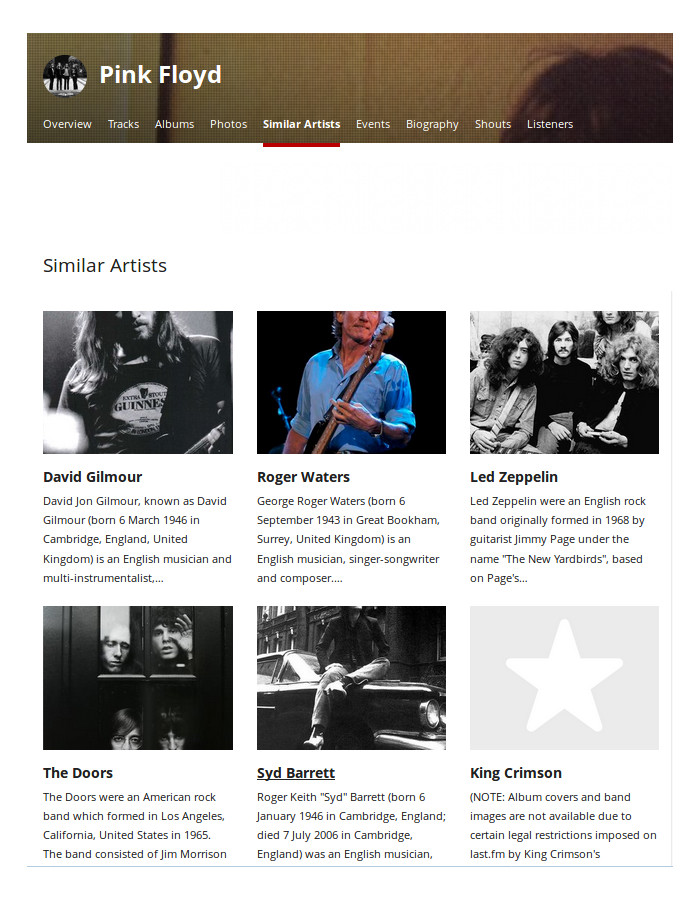
\includegraphics[width=7in,height=7in]{pics/lstfm-rs-example.jpeg}
\end{center}
\end{figure}

В момент решения задачи $topN$ и в момент проверки качества решения
в ООМ используется информация только
о тех объектах, для которых известно, что $(u_a \R i_0) \wedge (u_a \R
i_{\bot})$\footnote{
	Во-первых, данная информация является достаточной для решения задачи
	$topN$, а, во-вторых, информация о других значениях $\rho(u, i)$
	может быть недоступна. К примеру, для случая интернет-магазина, где
	существует только факт наличия приобретения товара без его оценки.
	},
поэтому при решении задачи $topN$ будем работать с множеством исходных
данных вида $P = \{(u, i, \rho(u, i)): u \R i \}$.

Правило вывода $\Pi_O$ ООМ для решения задачи $topN$ задается следующей формулой:
\begin{equation}
	\label{ors-pi-top}
	i \rt i_0 \Rightarrow (\rh(u_a, i) := 1) \wedge (u_a \R i)
\end{equation}
Значения $\rh(u_a, i)$ задаются равными единице, потому что тогда объекты $i$
будут близкими для активного пользователя при любом пороговом значении
$\Delta_{\R}$.
Правило вывода $\Pi_O$ говорит о том,
что если существует объект $i$, являющийся соседом для объекта $i_0$,
то, следуя эвристическому утверждению модели (\ref{assertORS1}), выполняется
отношение $u_a \R i$,
так как $u_a \R i_0$ по принятому для задачи $topN$ виду исходного множества.
То есть решение можно записать в форме утверждения: $(u_a \R i_0) \wedge (i \rt
i_0) \Rightarrow u_a \R i$.

Приведем схему решения задачи $topN$ при использовании правила вывода $\Pi_O$
(\ref{ors-pi-top}). Для того, чтобы составить множество объектов, между которыми и
активным пользователем выполняется отношение близости, по правилу вывода нужно найти объекты,
между которыми и объектами обучающего множества будет выполняться отношение
близости. Тогда, следуя эвристическому утверждению, между найденными объектами
и активным пользователем будет выполняться отношение близости: пусть $i \rt
i_0$, тогда, так как по виду исходного множества, принятого для задачи $topN$
выполняется $u_a \R i_0$, по эвристическому утверждению (\ref{assertORS1})
выполняется $u_a \rt i$ ---
$(u_a \R i_0) \wedge
(i \rt i_0) \Rightarrow u_a \rt i$, --- что и требуется по задаче $topN$.

Схему решения задачи $topN$ можно описать как формирование кластера
объектов $\nit = \{ i : i \rt I^a_0 \}$,
$|\nit| = N$, где
$I^a_0 = \{i_0: \rho(u_a, i_0) \in P_0\}$ --- центр кластера. Множество
объектов кластера (кроме центра) является искомым решением.

Определим способы задания отношения близости между объектом $i$ и
подмножеством объектов $I^a_0$
\label{deltaTneighbours}
 \cite{topn1,topn2,amazon-item2item,disser0}:
\begin{itemize}
	\item $I^a_0 \rt i \Leftrightarrow \Bigr( \frac{1}{|I^a_0|} \cdot \sum \limits_{i_0
		\in I^a_0} \di(i,i_0) \Bigl) \ge \Delta_i$.
		В стандартном решении  \cite{item-based} $topN$
		для определения меры близости между объектом $i$ и множеством объектов
		$I^a_0$ вычисляется сумма мер близости между объектом $i$ и объектами
		$i_0 \in I^a_0$.
		$I^a_0 \rt i \Rightarrow \Bigr( \frac{1}{|I^a_0|} \cdot \sum \limits_{I^a_0 \in I^a_0}
		\di(i,I^a_0)\Bigl) \ge \Delta_i \Rightarrow \exists$
$i_0 \in I^a_0, I^a_0 \rt i$.
По данным задачи и вследствие выполнения отношения $I^a_0 \rt i$, выполняется
		$(u_a \R I^a_0) \wedge (I^a_0 \R i) \Rightarrow u_a \R i$. Таким образом,
если объект $i$ принадлежит кластеру $\nit$ (то есть выполняется
		$I^a_0 \rt i$), то по утверждению ООМ  (\ref{assertORS1}) выполнится $u_a \R i$.
Поэтому данный способ определения отношения $i \rt I^a_0$ можно
		применять с правилом вывода $\Pi_O$ (\ref{ors-pi-top}) для решения задачи

\item $I^a_0 \rt i \Leftrightarrow$  $\exists I^a_0 \in I^a_0, I^a_0 \rt i$.
По данным задачи и способу задания $I^a_0 \rt i$ выполняется утверждение ООМ, то есть
		$(u_a \R I^a_0) \wedge (I^a_0 \rt i) \Rightarrow u_a \R i$.

Таким образом, если объект $i$ принадлежит кластеру $\nit$ (то есть $I^a_0 \rt i$),
		то по утверждению ООМ (\ref{assertORS1}) выполнится $u_a \R i$, что и требуется
от задачи.
Поэтому данный способ определения отношения $i \rt I^a_0$ можно
		применять с правилом вывода $\Pi_O$ (\ref{ors-pi-top}) для решения задачи
$topN$.
\end{itemize}
%%% Для вычисления значения меры близости между объектами системы может использоваться самая различная информация об объектах, которая
%%% зависит от реализации и предметной области РС\footnote{Поэтому при описании схемы, как 
%%% правило, не уделяется внимание контентам объектов}. К примеру, для кинематографической РС сценарий рекомендаций можно описать так: 
%%% если пользователь приобрел коллекцию DVD <<Крестный отец>>, то система может произвести рекомендации тех DVD, 
%%% где участвует Марлон Брандо, режиссером которых является Френсис Форд Коппола, или в жанре криминальная драма. 
%%% То есть характеристиками объекта может выступать любая
%%% известная и значительная информация о нем, в данном случае это: известный актер, режиссер и жанр.
%%--------------------------------------------
\bigbreak
Опишем один из вариантов исполнения ООМ и решим
задачу $topN$  \cite{item-based}.%TODO: set cite
\begin{itemize}
	\item $c_X(u_a) = (x_1, x_2, ..., x_|I|)$
		\begin{equation*}
			x_i =
			\begin{cases}
				1, &\text{если $u_a \R i$}\\
				0, &\text{иначе}
			\end{cases}
		\end{equation*}
		контент активного пользователя --- вектор {\it бинарных} оценок,
		отображающий информацию о том, какие объекты пользователь предпочитает.
		Примером такого контента является контент пользователя
		РС Amazon \cite{amazon-item2item}, где $x_i = 1$ означает то, что пользователь
		приобрел товар $i$;
	\item контент объекта в исследованиях РС, как правило,
		не определяется, так как множество характеристик объектов,
		их значений и структура контента не влияют на технику решения и могут
		варьироваться для различных реализаций РС. В описываемой модели
		воспользуемся векторным представлением, то есть
		$c_Y = (y_1,...,y_{|Y|})$;
	\item
		$\di(i,j) =\cos(\angle(c_Y(i),c_Y(j)))$.

		Типичной мерой близости, используемой при решении задачи $topN$ является
		косинус угла между контентами объектов, представляемых в виде векторов
		\cite{item-based,rs-handbook}.
	\item
		Чтобы не производить расчеты меры близости при формировании
		$\overline{P}^a_{\bot}$ каждый раз, когда активный пользователь
		делает запрос на решение задачи $topN$, значения мер близости $\di$
		рассчитываются заранее и заносятся в специальную матрицу $\mathbb{M}$
		размера $|I| \times |I|$:
		\begin{equation*}
			\mathbb{M}_{ij} =
			\begin{cases}
				\di(i,j), & i \ne j \\
				0, & \text{иначе}
			\end{cases}
		\end{equation*}

		Такой предварительный этап называется построением модели \cite{topn2}.
\end{itemize}

На рисунке (\ref{dia:matrix}) изображена блок-схема алгоритма
построения матрицы $\mathcal{M}$, которой соответствует псевдокод, представленный на изображении <<Алгоритм построения матрицы мер близости объектов>>  (\ref{alg:matrix})
\begin{figure}[htb]
	\caption{Блок-схема алгоритма построения матрицы $\mathcal{M}$}
\begin{center}
	\label{dia:matrix}
 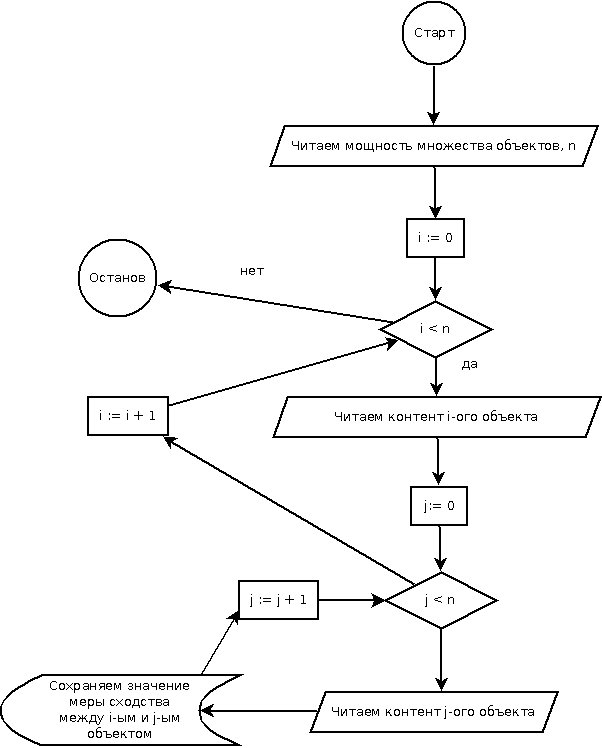
\includegraphics[width=6in,height=7in]{pics/algs/matrix.png}
\end{center}
\end{figure}

%\begin{figure}[htbp]
\begin{figure}[htb]
\caption{Алгоритм построения матрицы мер близости объектов}
\label{alg:matrix}
%\begin{algorithm}
\begin{algorithmic}[1]
\For{$i \gets 1, i \le n$}
	\State $\mathbb{M}_{ii} \gets 0$ \Comment{Чтобы пара с одинаковыми
	объектами не участвовала в дальнейших расчетах}
  \For{$j \gets 1, j \le n$}
  \State $\mathbb{M}_{ij} \gets \di(i,j)$
  \State $\mathbb{M}_{ji} \gets \mathbb{M}_{ij}$
  \State $j \gets j + 1$
  \EndFor
\State $i \gets i + 1$
\EndFor
\end{algorithmic}
%\end{algorithm}
\end{figure}

Для нахождения решения задачи $topN$ построим вектор
$\mathit{M} = (\overline{x}_1,...,\overline{x}_|I|)$, где
$
\overline{x}_i =
\begin{cases}
	0, &\text{если  $i \in I^a_0 $}\\
\mathbb{M}^i \times c_X(u_a)^T, &\text{ иначе }
\end{cases}
$\\
$c_X(u_a)^T$ --- транспонированный контент-вектор активного пользователя.
$I_{topN} = \{ i \in \{\overline{x}_i\} )\}$, где
$\{\overline{x}_i\}$ --- множество, состоящее из $N$ наибольших значений
координат вектора $\mathit{M}$.

На рисунке <<Блок-схема стандартного алгоритма решения задачи $topN$ в ООМ>> (\ref{dia:topn-solve-ors}) изображена блок-схема стандартного
алгоритма алгоритма решения задачи $topN$ в ООМ, которой соответствует
псевдокод, представленный на изображении <<Стандартный метод решения задачи $topN$ в ООМ>> (\ref{alg:topn-solve-ors})
\begin{figure}[htb]
	\caption{Блок-схема стандартного алгоритма решения задачи $topN$ в ООМ}
\begin{center}
	\label{dia:topn-solve-ors}
 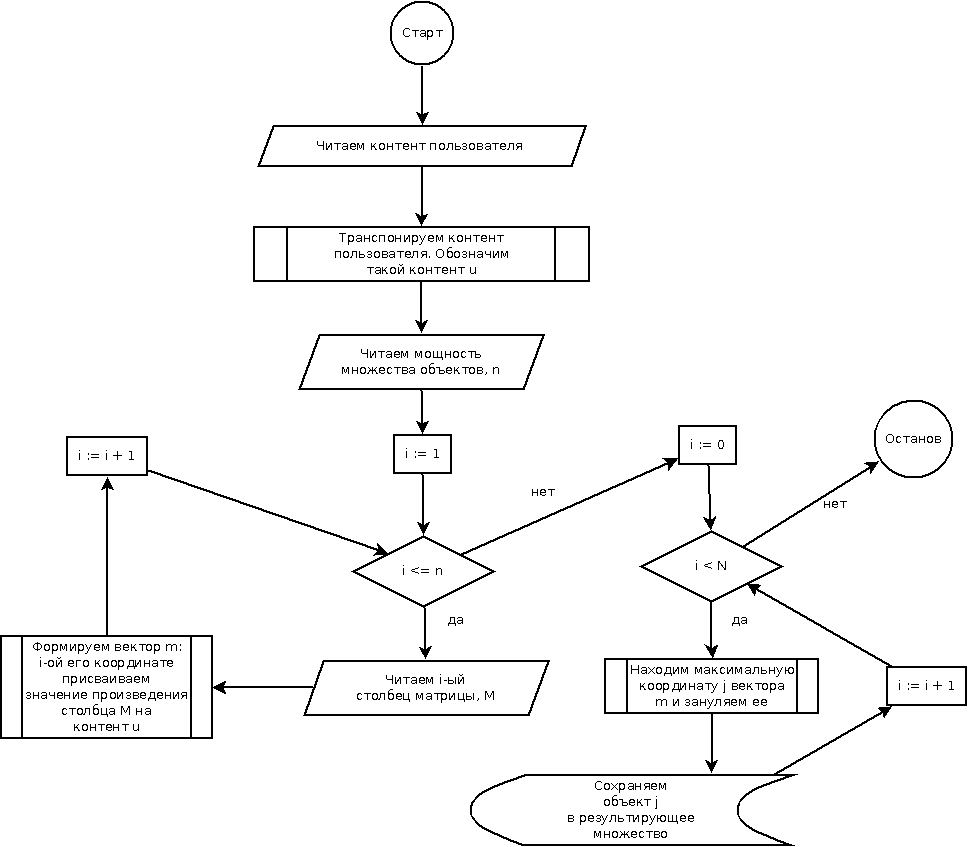
\includegraphics[width=7in,height=8in]{pics/algs/topn-ors.png}
\end{center}
\end{figure}

\begin{figure}[htb]
%\begin{algorithm}
\caption{Стандартный метод решения задачи $topN$ в ООМ}
\label{alg:topn-solve-ors}
\begin{algorithmic}[1]
\For{$i \gets 1, l \le n$} \Comment{Умножаем вектор-контент на матрицу}
	\State $m_i \gets \mathbb{M}^i \times c_X(u_a)^T$
\EndFor
\For{$j \gets 1, j \le N$}
	\State $i \gets \underset{i}{\mathrm{argmax}} \text{ } \overline{x}_i$
	\State $I_{topN} \gets I_{topN} \bigcup \{i\}$
	\Comment{Выбираем координату вектора $\mathit{M}$ с наибольшим значением}
\bigbreak
  \State $\overline{x}_i \gets 0$ \Comment{Зануляем уже выбранную координату}
  \State $j \gets j + 1$
\EndFor
\end{algorithmic}
%\end{algorithm}
\end{figure}


\subsubsection{Задача прогнозирования}
Эвристическое утверждение, на котором основывается решение задачи
$pred$ в ООМ, является более общим случаем утверждения
(\ref{assertORS1}):
\begin{assert}
	\label{assertORS2}
	Если два объекта схожи, то заданные им оценки близости пользователя будут
	приблизительно равны. \cite{rs-handbook,melville}.
\end{assert}
Данное утверждение является более общим случаем утверждения ООМ
(\ref{assertORS1}),
которое
используется при решении задачи $topN$,
так как рассматривает любые оценки, поставленные пользователем,
а не только те, которые означают, что между пользователем и объектом
выполняется отношение близости.

Во введенной терминологии данное утверждение примет следующий вид:
\begin{equation}
	i \rt j \Leftrightarrow |\rho(u,i) - \rho(u,j)|
	\le \varepsilon_p
\end{equation}

Правило вывода ООМ для решения задачи $pred$ запишется следующей
формулой:
\begin{equation}
	\label{ors-pi-p}
	\rh(u_a, i_{\bot}) = g_p(\{\rho(u_a, i^{\prime}_0)\}),
	i^{\prime}_0 \rt i_{\bot}.
\end{equation}
Правило вывода говорит о том, что оценки близости между
пользователем $u_a$ и объектами, являющимися соседями,
функционально связаны. Таким образом, зная
оценки близости, которые пользователь уже задал объектам
$i \rt i_{\bot}$, можно вычислить $\rh(u_a, i_{\bot})$
на основании функциональной связи
$g_p$.

Схема решения задачи $pred$ заключается в построении кластера
$\nip = \{ i_0 : i_0 \rt i_{\bot}\}$, центром которого является прогнозируемый
объект $i_{\bot}$. Решение задачи $pred$ запишется в виде:
\begin{equation}\label{pred-f}
	\rh(u_a,i_{\bot}) = g_p(\{\rho(u_a, i_0): i_0 \in \nip \}
\end{equation}
где $g_p$ --- некоторая функция, используемая в модели для
формирования по множеству оценок пользователя прогнозной оценки.

%===================================================================
%--------------------------------------------
%===================================================================
Опишем возможную\footnote{Модели могут отличаться такими параметрами, как,
например, функция $\di$, поэтому нижеописанная модель является одной из
возможных}
реализацию ООМ
\footnote{
	На данном этапе без оценки качества $\mathcal{E}_{topN}$
	}
 и на ее примере решим
задачу прогнозирования  \cite{item-based} %TODO: set cite. I think need
												%to see amazon
\begin{itemize}
	\item $c_X(u_a) = \{\rho(u_a,i_0)\}$
	\item $c_Y = (y_1,...,y_{|Y|})$;
	\item $\di(i,j) = \cos(\angle(c_Y(i),c_Y(j)))$
\end{itemize}
\bigbreak

Прогнозирование строится на основании оценок, поставленных активным пользователем
объектам, между которыми и прогнозируемым выполняется отношение близости.
Поиск таких объектов может осуществляться линейно по значениям, которые уже
хранятся в матрице мер близости $\mathbb{M}$, находящихся в строке с порядковым
номером, соответствующим индексу объекту. После построения кластера соседей
$\nip$,
вычисляется значение {\it прогнозной функции} от оценок пользователей,
поставленных $i \in \nip$.


На рисунке (\ref{dia:p-ors}) изображена блок-схема алгоритма
решения задачи $pred$ в ООМ.
\begin{figure}[htb]
	\caption{Блок-схема алгоритма построения матрицы $\mathcal{M}$}
\begin{center}
	\label{dia:p-ors}
 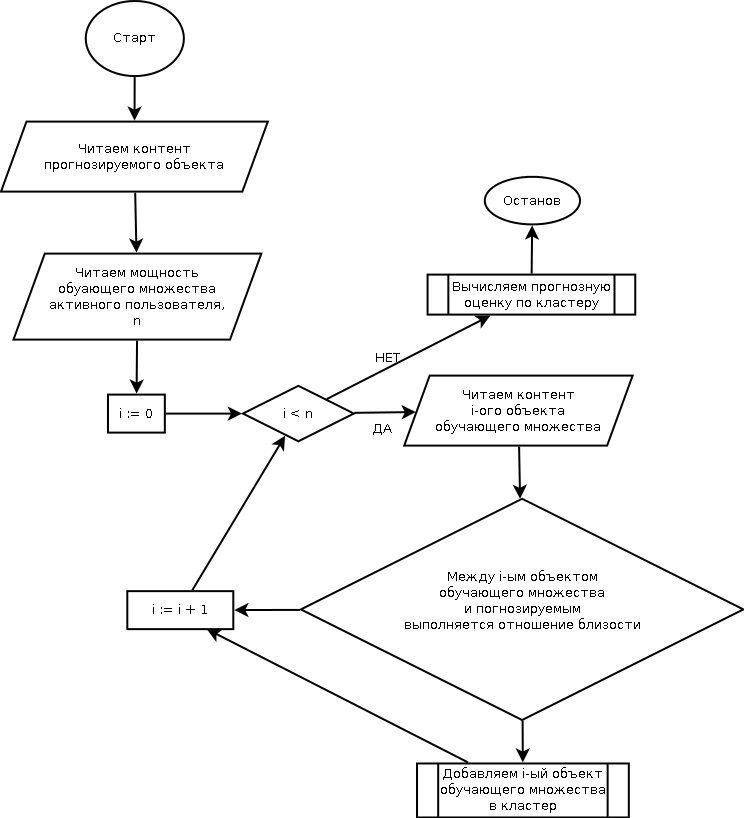
\includegraphics[width=7in,height=8in]{pics/algs/p-ors.png}
\end{center}
\end{figure}
Блок-схеме алгоритма решения задачи $pred$ в ООМ соответствует
псевдокод, представленный на изображении <<Стандартный алгоритм решения задачи $pred$ в ООМ>>  (\ref{alg:p-ors}).

\begin{figure}[htb]
\caption{Стандартный алгоритм решения задачи $pred$ в ООМ}
\label{alg:p-ors}
	%\begin{algorithm}
\begin{algorithmic}[1]
\State $\nip \gets \varnothing$\Comment{Множество объектов,
	оцененных активным пользователем и схожих с прогнозируемым объектом}
	\State $l \gets i_{\bot}$\Comment{Сохраняем в переменной $l$ индекс
	прогнозируемого объекта}
	\State $P^a \gets \varnothing$ \Comment{Множество оценок близости
	активного пользователя}
	\For {$i \in I^a_0$}
	\If {$\mathbb{M}^i_l \ge \Delta_i$}\Comment{Объект $i$ близок к
	прогнозируемому}
  \State $\nip \gets \nip \bigcup \{ i \}$
	\State $P^a \gets P^a \bigcup \{\rho(u_a,i)\}$
  \EndIf
\EndFor
\State $\rh(u_a,i) \gets g_p( P^a )$\Comment{Рассчитываем значение функции прогнозирования}
\end{algorithmic}
%\end{algorithm}
\end{figure}


\subsubsection{Функции вычисления прогнозной оценки}
Приведем
пример распространенной функции прогнозирования, применяемой в ООМ
 \cite{item-based}:
%cite
\begin{equation}\label{fpredict-ors}
	\frac{1}{|\nip|} \frac{\sum \limits_{i \in \nip} \di(i,i_{\bot}) \cdot \rho(u_a,i)}{
\sum \limits_{i \in \nip} \di(i,i_{\bot})
}
\end{equation}
%===================================================================
%--------------------------------------------
%===================================================================
\subsubsection{Используемые функции в качестве меры сходства}
\begin{itemize}
% ToDo: information retireval bib
\item \textbf{Косинус.} \newline
Наиболее популярная мера сходства, заимствованная из области
информационного поиска \cite{ir1,ir2,ir3}:
\begin{equation} \label{sim-cos}
	cos(\angle(c_Y(i),c_Y(j)) = \frac{\sum \limits_{k=1}^{|Y|} y^i_k \cdot y^j_k}{
		\sqrt{ \sum \limits_{k=1}^{|Y|} (y^i_k)^2 } \cdot
		\sqrt{ \sum \limits_{k=1}^{|Y|} (y^j_k)^2 }},
\end{equation}

\item {\bf Условная вероятность.} \newline
Данная мера сходства была разработана Кариписом \cite{topn1} для такой
предметной области РС, в которой оценки близости принадлежат бинарной
шкале. Оценки близости обладают семантикой условной вероятности
события (к примеру, приобретения товара),
которое зависит от истории поведения пользователя:
$Pr( \rho(u_a,i) = 1 | \rho(u_a,j) = 1 )$
\begin{equation}
Pr(i,j) = \frac{\tf(i \wedge j)}{\tf(i) \cdot \tf(j)^{\alpha}}
\end{equation}
где:
\begin{itemize}

\item $\tf(i)$ --- весовой коэффициент, использование которого заимствовано из
области информационного поиска, этот коэффициент определяет частоту
(от term frequency), с какой объект оценивается пользователями, то есть
$\tf(i) = |\{\rho(u,i): \rho(u,i) \in P_0\}|$,
$\tf(i ^ j) = |U^i \bigcup U^j|$,
$U^i = \{u: \rho(u_a,i) \in P_0\}$,
$U^j = \{u: \rho(u,j) \in P_0\}$.

\item $\alpha$ --- коэффициент, который служит для учета популярных объектов,
имеющих, к примеру, тенденцию быть приобретенными большинством пользователей
(и иметь, таким образом, большое значение частоты).

\end{itemize}

\item {\bf Коэффициент корреляции Пирсона.} Мера сходства,
заимствованная из статистики. Данная мера сходства использовалась
компаниями GroupLens \cite{grouplens} и Bellcore \cite{bellcore}.
\begin{equation}
 \frac{\sum \limits_{y}(y^1 - \overline{y^1}) \cdot (y^2 -
                                           \overline{y^2})}
                {\sqrt{\sum \limits_{y}(y^1 - \overline{y^1})^2 \cdot
        \sum \limits_{y}(y^2 - \overline{y^2})^2}},
\end{equation}

$\overline{y^k}$ -- среднее значение характеристики $k$-ого объекта.
\end{itemize}


\subsubsection{Примеры решения задач}
Рассмотрим примеры решения задач помощью ООМ.
\paragraph{Данные}
\begin{itemize}
\item
	Пусть контенты объектов некоторой системы представляют
		собой вектора в трехмерном пространстве характеристик $Y =
		\{y_1,y_2,y_3\}$, значения характеристик
	--- действительные числа.
	Пусть в системе существуют объекты со следующими контентами:
  \begin{enumerate}
  \item $c_Y(1) = (0,2; 0,8; 0)$;
  \item $c_Y(2) = (0; 1; 0)$;
  \item $c_Y(3) = (0,2; 1; 0)$;
  \item $c_Y(4) = (0; 0,2; 0)$;
  \item $c_Y(5) = (1; 0; 0)$;
  \item $c_Y(6) = (0,8; 0; 0)$;
  \item $c_Y(7) = (0; 0; 1)$;
  \item $c_Y(8) = (0; 0; 0,8)$;
  \item $c_Y(9) = (0; 0; 1)$;
  \end{enumerate}
\item Матрица мер сходства:\\
$\mathbb{M} = $
$
\begin{pmatrix}
0    & 0.97 & 0.99   & 0.97 & 0.24 & 0.19 & 0 & 0    & 0    \\
0.97 & 0    & 0.98   & 1    &   0  &  0   & 0 & 0    & 0    \\
0.99 & 0.98 & 0      & 0.97 & 0.58 & 0.19 & 0 & 0    & 0    \\
0.97 & 1    & 0.97   & 0    & 0.37 & 0    & 0 & 0    & 0    \\
0.24 & 0    & 0.58   & 0.37 & 0    & 1    & 0 & 0    & 0    \\
0.19 & 0    & 0.19   & 0    & 1    & 0    & 0 & 0    & 0    \\
0    & 0    & 0      & 0    & 0    & 0    & 0 & 0.98 & 1    \\
0    & 0    & 0      & 0    & 0    & 0    & 0.98 & 0 & 0.98    \\
0    & 0    & 0      & 0    & 0    & 0    & 1    & 0.98 & 0    \\
\end{pmatrix}
$
\item $c_X(u_a) = (1;1,0,0,0,0,1,0,0)$
\item $N = 2$ --- для задачи $topN$ нужно определить
	два объекта, между которыми и активным пользователем выполняется отношение
		близости;
\end{itemize}

\paragraph{Решение задачи $topN$}
\begin{enumerate}
\item В матрице $\mathcal{M}$ в каждом столбце оставляем $N$
	наибольших элементов:
$\mathcal{M'} = $
$
\begin{pmatrix}
0    & 0,97 & 0,99   & 0,97 &      & 0,19 & 0 & 0    & 0    \\
0,97 & 0    & 0,98   & 1    &   0  &  0   & 0 & 0    & 0    \\
0,99 & 0,98 & 0      &      & 0,58 & 0    & 0 & 0    & 0    \\
0    & 1    & 0      & 0    &      & 0    & 0 & 0    & 0    \\
0    & 0    & 0      & 0    & 0    & 1    & 0 & 0    & 0    \\
0    & 0    & 0      & 0    & 1    & 0    & 0 & 0    & 0    \\
0    & 0    & 0      & 0    & 0    & 0    & 0 & 0,98 & 1    \\
0    & 0    & 0      & 0    & 0    & 0    & 0,98 & 0 & 0,98    \\
0    & 0    & 0      & 0    & 0    & 0    & 1    & 0,98 & 0    \\
\end{pmatrix}
$
\item Перемножим {\it транспонированный} контент $c_X(u_a)^T$
	пользователя и матрицу $\mathcal{M'}$
		$m = (u_a)^T \times \mathcal{M'} = s = (0,97; 0,97, 1.97, 1.97, 0, 0,19, 0, 0,98, 1)$
\item Из вектора $m$ выбираем два наибольших значения. Им
	соответствуют объекты 3 и 4. Поэтому
		$I_{topN} = \{3, 4\}$.
\end{enumerate}

\paragraph{Задача прогнозирования}
Решим задачу прогнозирования для объекта 4 и активного пользователя со
следующими данными $P^a_0 = \{(2 | 1), (3, 0,1)\}$.
\begin{enumerate}
	\item $i_{\bot} = 4$ --- необходимо спрогнозировать оценку 4-ого объекта;
	\item Будем пользоваться функцией прогнозирования, описанной формулой
		(\ref{pred-f}).
	\item Составим множество соседей прогнозируемого объекта 4, для чего
		воспользуемся матрицей $\mathcal{M}$, $\nip = \{2, 3\}$
\item $\rho(u_a, 4) = \frac{1 \cdot 0.97 + 0,9 \cdot 1}{|0.97 + 1|} = 0,95$
\end{enumerate}

%===================================================================
%--------------------------------------------
%===================================================================
%===================================================================
%--------------------------------------------
%===================================================================

%-----------------------------------------------
%% \subsubsection{Примеры решения задач ООМ}
%% Рассмотрим примеры решения задач в ООМ. Будем использовать в примерах одни и те же данные
%% для каждой задачи, которые были описаны в разделе 1.3.6.

%% \paragraph{Задача top-$N$}
%% Решим задачу top-$N$ при $N=2$. Известно, что 
%% $I^a = \{ (i^1; 0,9), (i^2; 0,75), (i^5; 0,5), (i^6; 0,3), (i^{10}; 0,8)  \}$, поэтому контент активного пользователя
%% при решении задачи top-$N$ представляется в виде следующего вектора:
%% $a =
%% \begin{pmatrix} 
%% 1\\
%% 1\\
%% 0\\
%% 0\\.Ь = 
%% 0\\
%% 0\\
%% 0\\
%% 0\\
%% 0\\
%% 1\\
%% \end{pmatrix}
%% $
%% \begin{enumerate}
%% \item Предварительно проведем этап моделирование, в ходе которого построим матрицу оценок сходства $\mathbb{M}$
%% $
%% \begin{pmatrix} 
%% 0    & 0,99 & 0,76 & 0,47 & 0,62 & 0,07 & 0,98 & 0    & 0,26 & 0,7  \\
%% 0,99 &  0   & 0,74 & 0,5  & 0,69 & 0,14 & 0,96 & 0,08 & 0,35 & 0,74    \\
%% 0,76 & 0,74 & 0    & 0,8  & 0,39 & 0,31 & 0,85 & 0,21 & 0,24 & 0,1   \\
%% 0,47 & 0,5  & 0,8  & 0    & 0,63 & 0,81 & 0,55 & 0,74 & 0,69 &   0  \\
%% 0,62 & 0,69 & 0,39 & 0,63 & 0    & 0,71 & 0,54 & 0,7  & 0,91 & 0,91   \\
%% 0,07 & 0,14 & 0,31 & 0,81 & 0,71 & 0    & 0,08 & 0,99 & 0,92 & 0  \\
%% 0,98 & 0,96 & 0,85 & 0,55 & 0,54 & 0,08 & 0    &  0   & 0,21 &   0,57 \\
%% 0    & 0,08 & 0,21 & 0,74 & 0,7  & 0,99 & 0    &  0   & 0,92 &  0  \\
%% 0,26 & 0,35 & 0,24 & 0,69 & 0,91 & 0,92 & 0,21 & 0,92 & 0    & 0,37   \\
%% 0,7  & 0,74 & 0,1  & 0    & 0,91 & 0    & 0,57 &  0   & 0,37 & 0    \\
%% \end{pmatrix}
%% $

%% \item В полученной матрице в каждом столбце оставляем $N (=2)$ наибольших элементов:
%% $\mathcal{M'} = \\$
%% $
%% \begin{pmatrix} 

%% \end{pmatrix}
%% $
%% \item Перемножим {\it транспонированный} вектор-контент пользователя и матрицу, полученную в пункте 4:
%% $(u_a)^T \bot \mathcal{M'} = s = (0.97, 0.97, 1.97, 1.97, 0, 0.19, 0, 0.98, 1) \Rightarrow I^a_{topN} = \{i^3, i^4\}$
%% \end{enumerate}
%% \paragraph{Задача прогнозирования}
%% \begin{enumerate}
%% \item Из вида матрицы и условия\ref{example-cond}  следует, что что $\{i^1,i^2,i^3\}$ --- множество объектов, схожих с прогнозируемым;
%% \item $\rho(u_a, i^4) = \frac{1 \cdot 0.97 + 0.9 \cdot 1}{|0.97 + 1|} = 0.95$
%% \item Результат прогнозирования соответствует результату задачи top-$N$, так как $vp^a_l = 9.5 \Rightarrow a \R i$, и $i \in I^a_{topN}$
%% \end{enumerate}



%% \subparagraph{Характеристика объектно-ориентированных систем}
%% \subsubparagraph{Асимптотическая сложность решения и модели}
%% Для построения матрицы мер сходства необходимо вычислить $\frac{1}{2} \cdot (|T| - 1) \cdot |T|$ раз меру сходства. Сложность вычисления меры 
%% сходства зависит от мощности $C_T$. Однако $|CT| << |T|$, поэтому будем считать, что сложность вычисления меры сходства -- константа,
%% а {\bf асимптотическая сложность} определяется формулой $O(|T|^2)$.
%% {\bf  асимптотическая сложность} решения определяется умножением матрицы на вектор, она равна $O(|T|^2)$.

%% % ToDo сослаться на Сашину систему
%% Сложность данного решения велика, учитывая тот факт, что, как правило, в реальных систем $T$ огоромно. К примеру, 
%% новостная лента каждый день пополняет свою базу более, чем на 100 статей объектов. Таким образом, модель и решение
%% ООМ обладает {\it слабой масштабируемостью}.
%


%-----------------------------------------------


%%%\chapter{Субъектно-ориентированные эвристические коллаборативные системы}
\subsection{Субъектно-ориентированная модель рекомендательной
системы}
Одой из первых РС, в которой была применена
СОМ для решения задач, --- это РС, разработанная компанией
GroupLens \cite{grouplens}.

СОМ проводят анализ предпочтений
пользователей. Отфильтровываются те пользователи, чьи предпочтения не близки.
Если пользователи близки
по предпочтениям, то между ними выполняется отношение близости, и тогда
информация о таких пользователях используется для решения задачи. В
исследованиях, посвященных СОМ, такие пользователи называются
соседями \cite{neighbor-cf}.
Для РС интернет-магазина близость по предпочтениям может
выражаться, к примеру, тем, что пользователи приобретают одни и те
же товары (то есть объекты) \cite{e-commerce}.

В СОМ характеристиками пользователей являются объекты,
значениями характеристик --- значения $\rho(u, i)$, которые определяют
предпочтения пользователей.
В общем случае соседями считаются те пользователи,
кто одинаково оценивает одни и те же объекты, что во введенной
терминологии запишется в следующем виде:
\begin{equation}
	\label{user-sim1}
	u \ru v \Leftrightarrow \forall i: \exists \rho(u,i) \wedge
	\exists \rho(v,i) \text{ верно, что } |\rho(u,i) -
	\rho(v,i)| \le \varepsilon_p,
\end{equation}
где $\varepsilon_p$ --- некоторая малая фиксированная величина.

Определим отношение близости на основании меры близости
$\du: U \times U \rightarrow [0,1]$. Считается,
что если мера близости между пользователями больше некоторого порогового
значения, то пользователи являются соседями  \cite{threshold1, threshold2,
threshold3,threshold4,threshold5}:
\begin{equation}
	\label{user-sim2}
	u \ru v \Leftrightarrow \du(u,v) \ge \Delta_u, \Delta_u \in
	[0,1]
\end{equation}
Стоит отметить, что при разработке СОМ необходимо подбирать
параметры $\du$ и $\Delta_u$ так, чтобы близкие пользователи по определению
\ref{user-sim1}, были близки по определению \ref{user-sim2}:
важность подбора таким образом параметров будет описана в главах, посвященных
анализу коллаборативной фильтрации и последующих после текущей главы.

Правило вывода $\Pi_C$ в СОМ основано на утверждении, которое
гласит, что если в прошлом пользователи были близки по вкусам,
то и в будущем они будут близки по вкусам \cite{ub-assumption}.
Во введенной
терминологии данное утверждение примет следующий вид:
\begin{equation}
\label{srs-assert}
u_a \ru u \text{ выполняется на } P_0 \Rightarrow u_a
\ru u \text{ выполняется на } P_{\bot}
\end{equation}
Во время проведения тестов множеством будущего выступает тестовое множество,
множеством настоящего --- обучающее.

Правило вывода СОМ основывается
на эвристическом утверждении \cite{cfrs}, которое гласит :
\begin{assert}\label{assertSRS1}
пользователи, схожие по предпочтениям в прошлом, будут схожи и в будущем.
\end{assert}
Поэтому утверждение
во введенной терминологии запишется следующим образом:
\begin{equation*}
	\forall i_0:
	|\rho(u,i_0) - \rho(v,i_0)| \le \varepsilon_p
	\Rightarrow \forall i_{\bot} |\rho(u,i_{\bot}) - \rho(v,i_{\bot})|
	\le \varepsilon_p,
\end{equation*}

Правило вывода $\Pi_C$ в СОМ задается следующей формулой:
\begin{equation}
	\label{srs-pi}
	u \in U, (u_a \ru u) \Rightarrow |\rh(u_a, i_{\bot}) - \rho(u_a, i_{\bot})|
	\le \varepsilon_p, \rh(u_a, i_{\bot}) = f_p(\{\rho(u, i_{\bot})\}).
\end{equation}
Правило вывода СОМ говорит о том, что если пользователи $u$ являются
соседями для пользователя $u_a$, то оценки близости $\rho(u_a, i_{\bot}), \rho(u, i_{\bot})$
коррелируют, поэтому
неизвестное значение $\rho(u_a, i_{\bot})$ можно функционально определить по
значениям $\{\rho(u, i_{\bot})\}$, то есть прогнозная функция является функцией от
значений оценок близости соседей.

Данная модель используется, в основном, для решения задачи $pred$.
%Рассмотрим, как правило вывода применяется для решения задач.
%%%%%%%%%%%%%%%%%%%%%%%%%%% TOPN %%%%%%%%%%%%%%%%%%%%%%%%%%%%%%%%%%%%%%%%%%

\subsubsection{Задача $topN$}
Схема решения задачи $topN$ заключается в построении кластера соседей
$\nut = \{u: u_a \ru u\}$ активного пользователя $u_a$, который выступает в
роли центра кластера. После того, как кластер был
построен, выбирается $N$ объектов, которые близки для большинства
пользователей.

Это решение основано на правиле вывода $\Pi_C$ --- пусть объект $i$ близок
для большинства пользователей кластера $\nut$: $(\frac{1}{|\nut|} \sum \limits_{u \in
\nut} \rho(u,i)) \ge \Delta_{\R}$, а функциональная зависимость $f_p$
прогнозной функции $\rh$ определяется средним значением оценок близостей
соседей $\rho(u,i)$. Тогда $\rh(u_a, i) = f_p(\{\rho(u, i)\})
> \Delta_{\R}$, и тогда можно утверждать, что $u_a \R i$. $N$ таких объектов
составляет решение задачи $topN$.

Опишем возможную\footnote{Модели могут отличаться такими параметрами, как,
например, функция $\du$, поэтому нижеописанная модель является одной из
возможных}
модель CОМ
\footnote{
	На данном этапе без оценки качества $\mathcal{E}_{topN}$
	}
 и на ее примере решим
задачу $topN$  \cite{amazon-linden}.%TODO: set cite

\begin{itemize}
	\item $c_X(u_a) = (x_1, x_2, ..., x_n)$
\begin{equation*}
  x_i =
  \begin{cases}
	1, &\text{если $u_a \R i$}\\
	  0, &\text{иначе}
  \end{cases}
\end{equation*}
	Это распространенный способ представления контента,
	где координаты соответствуют объектам
		 \cite{topn1}.
	Данный способ представления
	информации о пользователях заимствован из информационного поиска
	 \cite{e-commerce,empirical-cf,ir4};
	\item $c_Y$ не определяется, так как с объектами в СОМ работа не проводится;
	\item $\di(u_a,u) =\cos(\angle(c_X(u_a),c_X(u)))$.
\end{itemize}

Чтобы сформировать кластер соседей, производится линейный поиск соседей
на множестве пользователей \cite{amazon-item2item}. Для построения результирующего
множества просуммируем контенты (данная операция
допустима, так как контент представляет из себя вектор) соседей,
и выберем те координаты $i$, которые обладают наибольшими значениями
и $(i, \rho(u_a,i)) \not \in P_0$.


На рисунке (\ref{dia:nut}) изображена блок-схема алгоритма
построения кластера соседей $\nut$, которой соответствует псевдокод
, представленный на изображении <<Построение множества соседей для активного
		пользователя $u_a$ при решении задачи $topN$>>
(\ref{alg:nut}).
\begin{figure}[htb]
	\caption{Блок-схема алгоритма построения кластера $\nut$}
\begin{center}
	\label{dia:nut}
 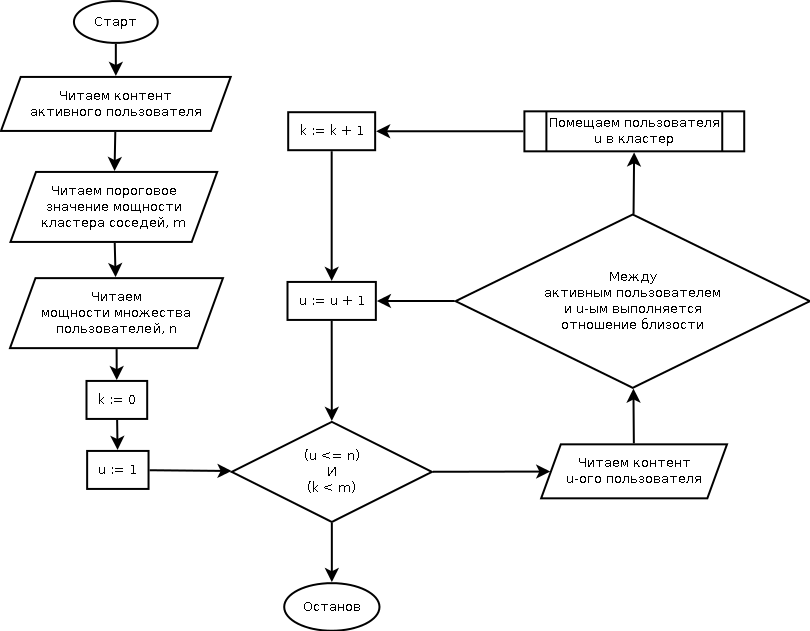
\includegraphics[width=7in,height=8in]{pics/algs/nut.png}
\end{center}
\end{figure}

\begin{figure}[htbp]
	%\begin{algorithm}
		\caption{Построение множества соседей для активного
		пользователя $u_a$ при решении задачи $topN$}
		\label{alg:nut}
		\begin{algorithmic}[1]
			\State $\nut \gets \varnothing$
			\State $k \gets 0$
			\For {$u \gets 1 \to |U|$}
			\If{$u_a \ru u$}
			\State $\nut \gets \nut \bigcup \{ u \}$
			\State $k \gets k + 1$
			\EndIf
			\If{$k > M$}\Comment{Ограничение на размер множества соседей}
			\State Стоп
			\EndIf
			\EndFor
		\end{algorithmic}
	%\end{algorithm}
\end{figure}


На рисунке (\ref{dia:topn-srs}) изображена блок-схема решения задачи $topN$ в
$COM$, которой соответствует псевдокод, представленный на изображении <<Стандартный алгоритм решения задачи $topN$>>  (\ref{alg:topn-srs}).
\begin{figure}[htb]
	\caption{Решение задачи $topN$ в $COM$}
	\begin{center}
		\label{dia:topn-srs}
		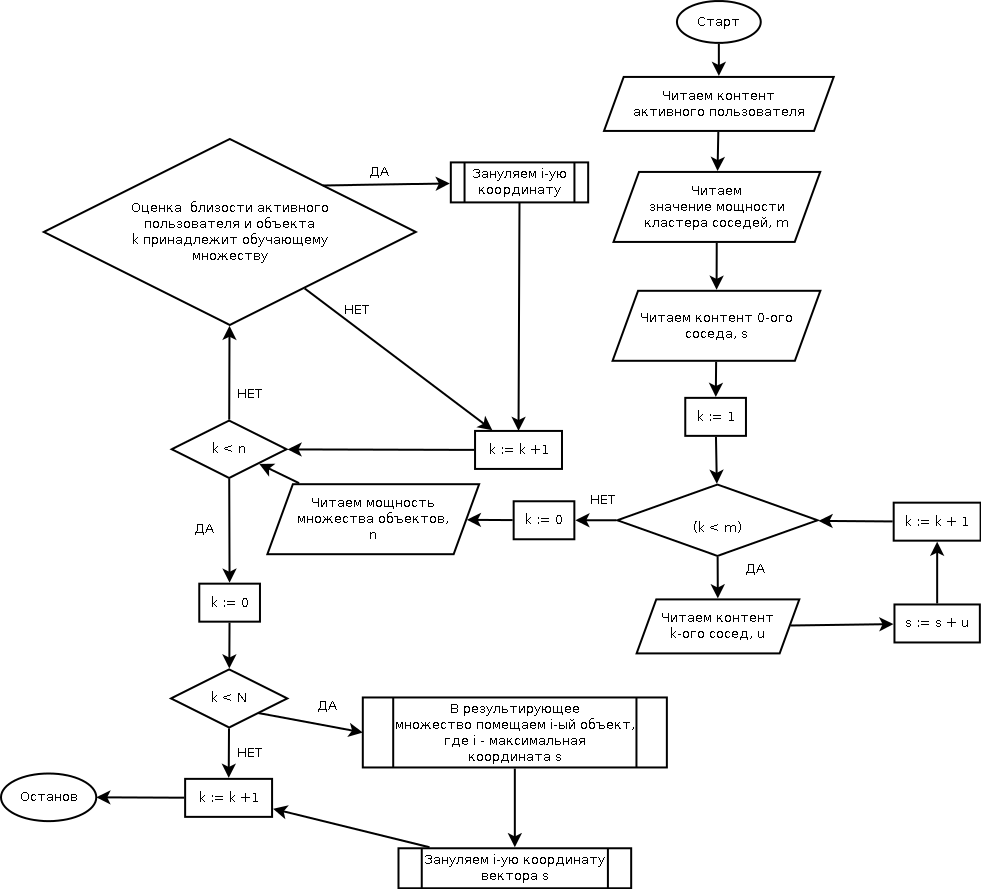
\includegraphics[width=7in,height=8in]{pics/algs/topn-srs.png}
	\end{center}
\end{figure}

\begin{figure}[htbp]
	%\begin{algorithm}
		\caption{Стандартный алгоритм решения задачи $topN$}
		\label{alg:topn-srs}
		\begin{algorithmic}[1]
			\State $s \gets \sum \limits_{u \in \nut} u$ \Comment{Вектор-сумма}
			\For {$i \gets 1, i \le |I|$}
			\If {$\exists \rho(u_a,i)$} \Comment{Если активный пользователь уже оценил
			объект, то он должен отсутствовать в результирующем множестве}
			\State $s_i \gets 0$ \Comment{Зануляем $i$-ую координату}
			\EndIf
			\EndFor
			\State $\overline{P}^a_{\bot} \gets \varnothing$
			\State $I_{topN} \gets \varnothing$
			\For {$k \gets 1, k \le N$}
			\State $i \gets \underset{i} {\mathrm{\max}}$ $s$
			\State $I_{topN} \gets I_{topN} \bigcup \{i\}$
			\State $\overline{P}^a_{\bot} \gets \overline{P}^a_{\bot} \bigcup
			\{ 0 \}$ \Comment{Для решения задачи нужно составить множество объектов, а не
			определить близость, поэтому $\rho(a,i)=0$, так как тогда $\forall
			\epsilon_0:$ $u_a \R i$}
			\State $s_i \gets 0$
			\State $k \gets k + 1$
			\EndFor
		\end{algorithmic}
	%\end{algorithm}
\end{figure}


\subsubsection{Задача прогнозирования}
Подобно задаче $topN$, для решения задачи $pred$ \cite{cfrs, cf-expert,
rs-handbook, toward,coscial-rec-survey, user-item-cf,rs-cf}
строится кластер соседей, центром которого является активный пользователь
$u_a$, однако в кластер входят не только те пользователи, между которыми
и активным выполняется отношение близости, но и такие, которые оценили
прогнозируемый объект $i_{\bot}$:
$\nup = \{u: u_a \ru u \wedge \rho(u,i_{\bot}) \in P_0\}$. Такое дополнительное
условие накладывается для того, чтобы по известным $\rho(u, i_{\bot}), u \in \nup$
определить неизвестную $\rho(u,i_{\bot})$.
Следуя утверждению СОМ (\ref{assertSRS1}), $\forall$ $u \in \nup$ выполняется $|\rho(u_a,i_{\bot}) -
\rho(u,i_{\bot})| \le
\varepsilon_p$.
Для того, чтобы рассчитать прогнозную оценку,
вычисляется значение некоторой прогнозной функции $f_p$
от оценок, поставленных прогнозируемому объекту соседями:
\begin{equation}
	\rh(u_a,i_{\bot}) = f_p(\{ \rho(u,i_{\bot}): u \in \nup \})
\end{equation}

На рисунке (\ref{dia:nup}) изображена блок-схема алгоритма
построения кластера соседей $\nup$, которой соответствует псевдокод
(\ref{alg:nup}).
\begin{figure}[htb]
	\caption{Блок-схема алгоритма построения кластера $\nup$}
\begin{center}
	\label{dia:nup}
 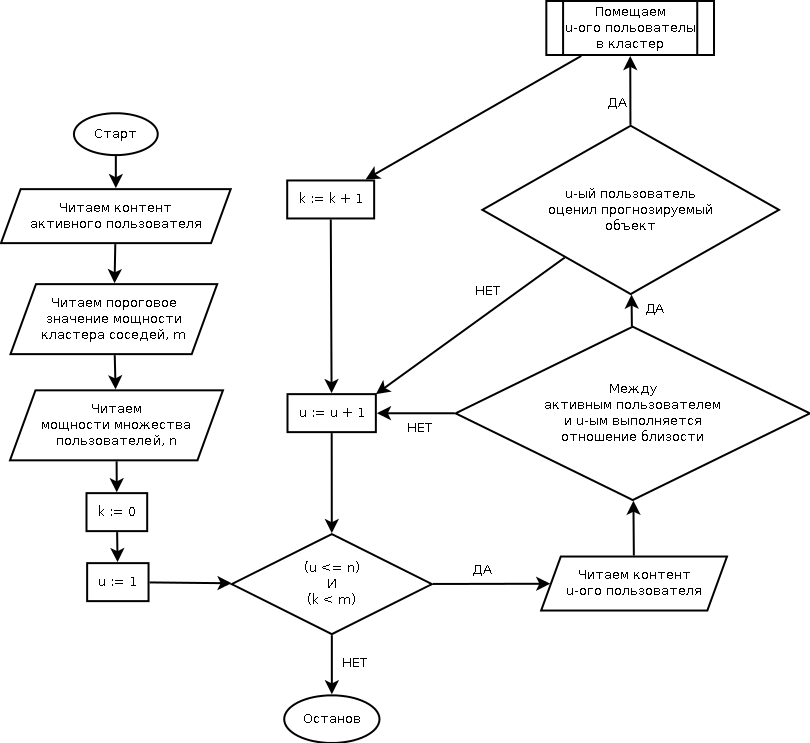
\includegraphics[width=7in,height=8in]{pics/algs/nup.png}
\end{center}
\end{figure}

\begin{figure}[htb]
	%\begin{algorithm}
		\caption{Построение множества соседей для активного
		пользователя при решении задачи прогнозирования в СОМ}
		\label{alg:nup}
		\begin{algorithmic}[1]
			\State $\nup \gets \varnothing$
			\State $k \gets 0$
			\For {$u \gets 1 \to |U|$}
			\If{($u_a \ru u$) $\wedge$ $(\exists$ $\rho(u, i_{\bot}))$}
			\State $\nup \gets \nup \bigcup \{ u \}$
			\State $k \gets k + 1$
			\EndIf
			\If{$k > M$}\Comment{Ограничение на размер множества соседей}
			\State Стоп
			\EndIf
			\EndFor
		\end{algorithmic}
	%\end{algorithm}
\end{figure}

Стандартный алгоритм решения задачи $pred$ в СОМ производится
в две итерации, которым соответствует псевдокод, представленный на изображении <<Стандартный алгоритм решения задачи прогнозирования в СОМ>>
 (\ref{alg:p-srs}):
\begin{enumerate}
	\item формирование кластера соседей $\nup$ (\ref{alg:nup});
	\item вычисление прогнозной функции по множеству оценок $\{\rho(u, i_{\bot}): u
		\in \nup\}$.
\end{enumerate}

\begin{figure}[htb]
	\caption{Стандартный алгоритм решения задачи прогнозирования в СОМ}
	\label{alg:p-srs}
		\begin{algorithmic}[1]
			\State $\nup$ \Comment{Формируем кластер соседей}
			\State $\rh(u_a, i_{\bot}) \gets f(\{\rho(u, i_{\bot}): u
			\in \nup\})$ \Comment{Вычисляем прогнозную функцию}
		\end{algorithmic}
\end{figure}


\subsubsection{Функции вычисления прогнозной оценки}
Приведем примеры распространенных функций $f_p$, которые используются для
вычисления значения прогнозной функции по значениям $\rho(u, i), u \in \nup$.
\begin{itemize}
  \item Среднее  \cite{surveyCf}:
  \begin{equation}
	\label{middle-pred}
    \frac{1}{|\nup|} \cdot \sum \limits_{u \in \nup} \rho(u,i_{\bot}).
  \end{equation}
  \item Среднее взвешенное \cite{surveyCf}:
  \begin{equation}
	  \label{weighted-pred}
    \overline{\rho^a} +
    \frac{ \sum \limits_{u \in \nup} \du(u_a,u) \cdot (\rho(u,i_{\bot}) -
	  \overline{\rho^u}) }
{ \sum \limits_{u \in \nup} | \du(u_a,u) | }
  \end{equation}
  $\overline{\rho^a}$ --- среднее значение близости активного пользователя,
		$\overline{\rho^u}$ --- среднее значение близости пользователя $u$.
Вычитание средней оценки близости призвано устранить эффект,
который накладывается от характера пользователя:
		лояльные пользователи ставят оценки близости не ниже определенной,
строгие пользователи --- наоборот \cite{norm, rs-handbook}.

Приведенные способы вычисления прогнозной оценки являются распространенными, но не единственными.
К примеру, компания Ringo \cite{ringo} не использовала в своей системе веса,
а среднее значение меры сходства соседей. Однако
метод среднего взвешенного является не только простым и распространенным,
но и согласуется с
теорией общественного выбора, ее обоснованиями человеческого поведения, ---
первичными принципами коллаборативной фильтрации  \cite{cfrs,bellcore}.
\end{itemize}

%%%%%%%%%%%%%%%%%%%%%%%%%%%%%%%%%%%%%%%%%%%%%%%%%%%%%%%%%
\subsubsection{Меры сходства}
Приведем примеры распространенных функций, которые используются в качестве меры
сходства.
\begin{itemize}
\item Коэффициент корреляции Пирсона\label{pearson}:
\begin{equation}
	\du(u,v)\frac{\sum \limits_{i \in I_{\bigcap}}(\rho(u,i) - \overline{\rho}^u) \cdot
	(\rho(v,i) - \overline{\rho}^v)}
                {\sqrt{\sum \limits_{i \in I^u}(\rho(u,i) - \overline{\rho})^u \cdot
                    \sum \limits_{i \in I^v}(\rho(v,i) - \overline{\rho}^v)^2}}
\end{equation}
\begin{equation*}
	I^a = \{i: (i, \rho(a,i)) \in P^a_0\}, a \in \{u,v\},P^a_0 = \{\rho(a, i_0)\}
\end{equation*}
\begin{equation*}
	I_{\bigcap} = I^u \bigcap I^v
\end{equation*}
\item Косинус угла между контентами.
	Для применения этой меры сходства необходимо представлять
контенты как элементы векторного пространства, в котором координата
		соответствует объекту и равна нулю, если пользователь не оценивал
		данный объект.
\begin{equation}
cos(\angle(u,v) = \frac{\sum \limits_{ i \in I_{\bigcap} } \rho(u,i) \cdot \rho(v,i)}{
\sqrt{ \sum \limits_{i \in  I^u } (\rho(u,i))^2 } \cdot \sqrt{ \sum \limits_{ i \in I^v} (\rho(u,i))^2 }},
\end{equation}
\end{itemize}


\subsubsection{Примеры решения задач}
Рассмотрим примеры решения задач в СОМ.
\paragraph{Данные}
\begin{itemize}
\item $N=2$ --- для задачи $topN$ требуется определить 2 топовых объекта;
\item $i_{\bot} = 7$ --- для задачи прогнозирования необходимо спрогнозировать оценку на объект 7;
\item $\mathcal{S} = \{0,1;0,2;0,3;0,4;0,5\}$ --- оценки принадлежат относительной шкале от 1 до 5. Если оценка равна 0; то пользователь не
ставил оценку на данный объект.
\item $|I| = 10$
\item Контенты пользователей --- вектор оценок, где $i-ая$ координата соответствует $i$-ому объекту.
  \begin{itemize}
    \item $a =   (0,5; 0,2; 0,4; 0,3; 0,5; 0,0; 0,0; 0,0; 0,0; 0,0)$
    \item $u_1 = (0,5; 0,2; 0,5; 0,0; 0,4; 0,2; 0,5; 0,0; 0,0; 0,0)$
    \item $u_2 = (0,4; 0,3; 0,5; 0,0; 0,4; 0,0; 0,0; 0,4; 0,5; 0,2)$
    \item $u_3 = (0,2; 0,5; 0,2; 0,4; 0,3; 0,0; 0,0; 0,5; 0,4; 0,0)$
    \item $u_4 = (0,0; 0,0; 0,0; 0,0; 0,0; 0,2; 0,0; 0,3; 0,5; 0,5)$
    \item $u_5 = (0,4; 0,2; 0,0; 0,0; 0,4; 0,2; 0,5; 0,5; 0,0; 0,0)$
  \end{itemize}
\item $\Delta_{\R} = 0,49$
\item В качестве меры сходства будем использовать коэффициент корреляции
	Пирсона (\ref{pearson}).
\item
  \begin{equation}
    \du(u_1,u_2) > 0.8 \Rightarrow u_1 \ru u_2
  \end{equation}
\end{itemize}
\paragraph{Задача $topN$}
\begin{enumerate}
\item Составим множество соседей мощности 2. Для этого рассчитаем меру сходства между активным пользователем и другими:
  \begin{itemize}
  \item $\du(u_a,u_1) = 0,94 \Rightarrow u_1 \in \nut$
  \item $\du(u_a,u_2) = 0,57$
  \item $\du(u_a,u_3) = -0,85$
  \item $\du(u_a,u_4) = \varnothing$
  \item $\du(u_a,u_5) = 0,81 \Rightarrow u_5 \in \nut$
  \end{itemize}
\item $s = \sum \limits_{u \in \nut} u = (0,9; 0,4; 0,5; 0,0; 0,8; 0,4; 1,0; 0,5; 0,0; 0,0)$
\item Зануляем значения координат, для которых $\rho(u_a, i) \in P_0: s =
	(0,0; 0,0; 0,0; 0,0; 0,0;0,4; 1,0; 0,5; 0,0; 0,0)$
\item $I_{topN} = \{ 7, 8 \}$
\end{enumerate}
\paragraph{Задача прогнозирования}
При решении предыдущей задачи было составлено множество соседей.
Определим прогноз по оценкам этих соседей:
\begin{equation}
f_p(u_a,7) =  0,38 + \frac{ 0,94 \cdot (0,5 - 0,38) + 0,81 \cdot (0,5 - 0,36)}{
	0,94 + 0,81 } = 0,55
\end{equation}

%%%%%%%%%%%%%%%%%%%%%%%%%%% PREDICT %%%%%%%%%%%%%%%%%%%%%%%%%%%%%%%%%%%%%%%%%%
%%%%%%%%%%%%%%%%%%%%%%%%%%% PREDICT FUNCTIONS %%%%%%%%%%%%%%%%%%%%%%%%%%%%%%%%%%%%%%%%%%

%eval-sim-metrics ToDo: раписать целевую
\section{Описание функций оценок качества решений задач} \label{def-eval}

\subsection{Оценка решения задачи прогнозирования}
Данные оценки определяют, насколько {\it аккуратно} был произведен прогноз путем
расчета погрешности между спрогнозированной оценкой близости и реальной,
принадлежащей тестовому множеству.

Приведем распространенные оценки эффективности этого класса:
\begin{itemize}
\item
  \begin{equation}
	  MAE = \frac{1}{|P^a_{\bot}|} \sum \limits_{(u_a, i_{\bot}, \rho(u_a,
	  i_{\bot})) \in P^a_{\bot}} |\rho(u_a, i_{\bot})
	  - \rh(u_a, i_{\bot})|,
  \end{equation}
		где $P^a_{\bot} = \{\rho(u_a, i_{\bot})\}$ --- тестовое множество
		активного пользователя;
\item
  \begin{equation}
	  \label{nmae}
	  NMAE = \frac{1}{|P_{\bot}|} \cdot (\rho_{\max} - \rho_{\min})
	  \sum \limits_{i \in I_{\bot}} |\du(u_a, i^m_{\bot}) - \rho(u_a, i^m_{\bot})|,
  \end{equation}
$\rho_{\max}, \rho_{\min}$ --- максимальная и минимальная оценки
шкалы соответственно.

Значения $NMAE$ труднее интерпретировать по отношению к масштабу шкалы,
но они сопоставимы для шкал любого масштаба.
\item
  \begin{equation}
	  RMSE = \sqrt{\frac{1}{|P^a_{\bot}|} \sum \limits_{(u_a, i_{\bot}, \rho(u_a, i_{\bot})) \in P^a_{\bot}}
	  (\rh(u_a, i_{\bot}) - \rho(u_a, i_{\bot}))^2}
  \end{equation}
\end{itemize}

%Решение задачи прогнозирования можно рассматривать как формирование системой
%прототипа пользователя $\overline{a}$,
%в контент которого входят спрогнозированные значения.
%Тогда цель системы заключается в том, чтобы сформировать контент пользователя
%$\overline{a}$ так, что
%$a \ru \overline{a}$, то есть $\forall i_{\bot}$ $|\rho(u_a,i_{\bot}) -
%\overline{\rho}(\overline{a},i_{\bot})| \le \epsilon_0$,
%$\overline{\rho}(u_a,i_{\bot})$ --- спрогнозированная оценка.
%Но тогда и оценки эффективности будут иметь значение меньше либо равное
%$\epsilon_0$. Поэтому будем говорить, что решение эффективно, если
%значение оценки эффективности меньше либо равно $\epsilon_0$.

\subsection{Оценка решения задачи $topN$}
% ToDo добавить еще P@ и всякие NDCG
Делая запрос на решение задачи $topN$, активный пользователь $u_a$
ставит перед системой цель
определить множество $I_{topN}$ таких объектов $i$, что $u_a \R i$. Для того,
чтобы определить, насколько точно по отношению к цели было составлено множество
$I_{topN}$ применяются функции, именуемые оценками точности. Эти функции можно
описать как функции, которые сравнивают результирующее
множество с тестовым и определяют качество как точность \lq попадания \rq
объекта из результирующего множества в тестовое.
Эти функции заимствованы из области информационного поиска \cite{ir1,ir2,ir3}.
При оценке задачи $topN$ состоит из объектов, между которыми и активным
пользователем выполняется отношение близости, как и при решении задачи:
$P^a_{\bot} = \{ (u_a,  i_{\bot}, \rho(u_a, i_{\bot})): u_a \R i_{\bot}\}$.

Для определения используемых оценок точности введем функцию,
которая определяет, выполняется ли отношение $u_a \R i$:
$
s(i) =
\begin{cases}
1, &\text{$\exists$ $i_{\bot} \in I_{\bot}$: $u_a \R i_{\bot}$}\\
0, &\text{иначе}.
\end{cases}
$\\

Функция $s$, заданная таким образом соответствует цели пользователя, поэтому
оценки точности, которые определены на базе такой функции $s$ будем называть
{\it целевыми}.

Приведем пример целевых оценок точности:
\begin{itemize}
\item Точность:
	\begin{equation}
		\label{precision}
	1 - \frac{1}{N} \cdot \sum \limits_{i \in I_{\bot}} s(i);
	\end{equation}
%\item Полнота: $1 - \frac{1}{M} \cdot \sum \limits_{i \in I_{\bot}} s(i)$,
%где $M = \{|i \in \mathbb{N}^n : a \R i |\}$ ---
%число всех объектов множества $I$, для которых выполняется отношение
%близости с активным пользователем. Как правило, полнота оценивается на
%объединении результирующих множеств, полученных на большом числе тестов
%или при $N \approx M$. Будем считать, что для полноты $M = N$\label{recall-meqn};
\item Точность $P@L$ для списка объектов длины $L$:
\begin{equation}
1 - \frac{1}{L} \cdot \sum \limits_{i \in I_L} s(n),I_L \subset I_{\bot},
|I_L| = L.
\end{equation}
\item
	\begin{equation}
	AveP = \frac{1}{\sum \limits_{n=1}^{N} s(n)} \cdot
\sum \limits_{L=1}^{N},
\end{equation}
		где $P@L$ --- среднее значение $P@L$ для $L=1..N$.
	\item
		\begin{equation}
		NDCG = 1 - \frac{DCG}{IDCG},
		\end{equation}
			где $DCG = s(1) + \sum \limits_{k=1}^N
\frac{s(i_k)}{log_2(i_k)}$ --- сумма <<весов накопления>>,
где <<вес накопления>> зависит от порядкового номера
в ранжированном результирующем множестве.
Чем меньше порядковый номер объекта,
между которым и активным пользователем выполняется отношение
близости, тем результат качественней, а вес объекта больше.
		Данная оценка используется, к примеру, для поисковых систем\cite{},
		где для пользователя важно, чтобы интересующий его объект находился в
		начале результирующего списка.
\end{itemize}

Однако, совместно с ООМ эти оценки не могут использоваться, так как ООМ
не определяют функцию $\rho: U \times I$. Вместо нее используются значения
прогнозной функции, которые рассчитываются на основании правил вывода ООМ.
Подобно решению, оценка решения задачи $topN$ при применении ООМ,
основана на эвристическом утверждении (\ref{assertORS1}). Чтобы определить,
является ли объект $i \in I_{topN}$ целевым по отношению к поставленной задачи,
нужно выяснить, существует ли объект обучающего множества, являющийся соседом
для объекта $i$. Так как для объектов обучающего множества верно, что $u_a \R
i_0$, то по эвристическому утверждению (\ref{assertORS1}) получим, что $u_a \R
i$, так как $i \rt i_0$.

Для определения качества решения в ООМ используются те же целевые функции,
но их значения зависят не от функции $s$, а от функции $\overline{s}$:
$
\overline{s}(i) =
\begin{cases}
	1, &\text{$\exists$ $i_{\bot} \in I_{\bot}$: $i \rt i_{\bot}$}\\
0, &\text{иначе}.
\end{cases}
$\\
Такие оценки точности будет называть {\it объектно-ориентированными}.

